%# -*- coding: utf-8-unix -*-
%%==================================================

\chapter{Other Guides}

\begin{flushright}
    ——Take a glance, no loss; take a second look, huge gain
\end{flushright}

\section{大坑:假如明天你突然丢失电脑所有数据怎么办?——如何备份资料}

\begin{figure}[H]
    \begin{tabular}{rl}
        
\includegraphics[width=0.5\columnwidth]{author-folder/Kai.Wu/backup1.jpg} &
        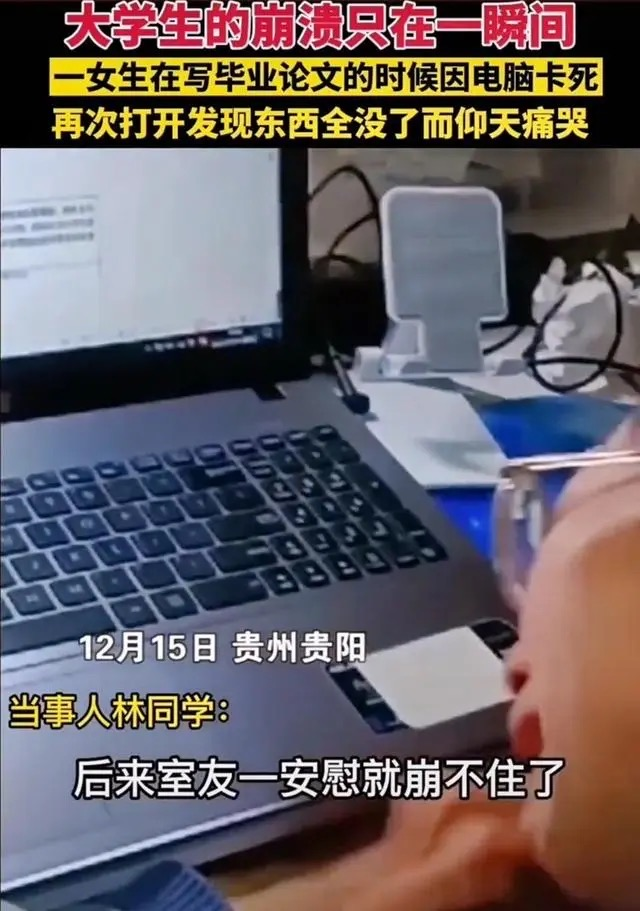
\includegraphics[width=0.4\columnwidth]{author-folder/Kai.Wu/backup2.jpg}
    \end{tabular}
    \caption{\href{https://baijiahao.baidu.com/s?id=1719578217211021768}{链接:贵阳一女大学生8000字毕业论文保存失败崩溃大哭}}
\end{figure}

绝大部分同学本科就买了自己的电脑。虽然自己的各种作业资料,到现在博士阶段的研究数据、论文,全部就只存放在这一台电脑里,但并没有足够意识到自己电脑的重要,和保存在电脑里信息的脆弱。每年,都会有如上图的事情发生,给当事人带来上新闻被全国人民笑话的沉重打击。

丢失一篇正在写的论文,其实是小事,毕竟研究资料全部都在。上面新闻的当事人,其实也就用了几天时间就重新写好了论文。但那些万年不动、又极其重要的资料,又是绝对安全的吗?

想象一下,假如
\begin{itemize}
    \item 你某天手一滑,电脑摔倒地上,再也开不了机,硬盘也没法恢复
    \item 头昏脑涨的一天,你接了一杯咖啡,一不注意,咖啡撒在了电脑上,瞬间短路,电脑滋滋冒油
    \item 你不慎点击了一个链接,中了勒索病毒;或者,西浦内网被网络攻击攻陷,所有电脑中勒索病毒。你的所有文件被加密封锁。
    \item 你把电脑带出去办公或者采集数据,整个电脑直接被偷走
    \item 你过年回家,在路上,背包或者行李箱被人偷走了或者拿错了
    \item 无恶意,但万一,西浦着火了,西浦进水了(MB的5楼一下大雨就漏水),西浦楼塌了,撤离的时候你根本来不及拿电脑
\end{itemize}


\begin{figure}[H]
    \centering
    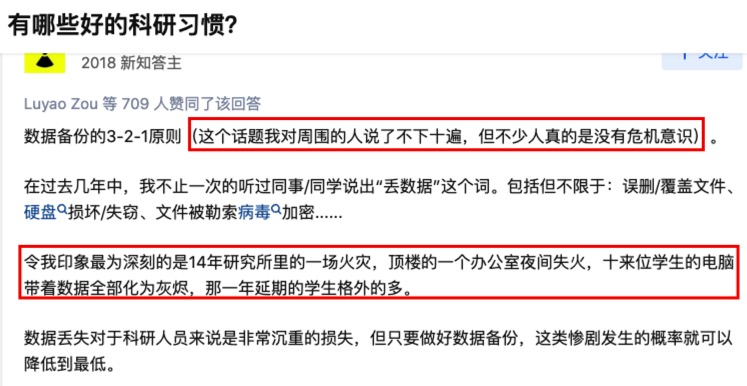
\includegraphics[width=0.8\columnwidth]{author-folder/Kai.Wu/backup_zhihu.jpg}
    \caption{\url{https://www.zhihu.com/question/394796969/answer/1501840215}}
\end{figure}

这些情况,单个可能很罕见,但所有可能性加起来,再乘以3到4年时间,至少发生一次的概率并不小。如果发生,你的博士进度会被耽误多久,你的青春又会被耽误多久呢。

只有一份的数据是非常脆弱的。现在思考一下,你赖以生存的电脑、数据、论文,是否只存了一份?如果是,请立即把屁股从椅子上挪起来,去厕所洗把脸,问问自己都是成年人了,怎么心这么大,然后开始看下面的攻略。

\subsection{理论:321原则}

「3-2-1 原则」是商业公司通用的数据备份金方法,具体内容是:
\begin{itemize}
    \item 3:存储 3 份完整文件,一份原件加上两份拷贝。
    \item 2:将文件起码保持在两种不同的介质上。
    \item 1:将一份拷贝保存在异地。
\end{itemize}

所谓的「介质」,是指内置硬盘、移动硬盘、U盘、网盘等不同的存储介质。说起来好像很麻烦,但对我们来说最简单的实践是:原件保存在内置硬盘,将两份拷贝分别存到移动硬盘和网盘,就同时达成了三条要求。这时,你回过头去看一下我上面列举的所有可能的灾难性问题(甚至即使是网盘公司突然倒闭),都能做到游刃有余,不影响你的科研!

\subsection{实践}

到动手准备的环节了。首先根据你手里的资源,决定你要备份的范围。最土豪的情况,你可以把整个电脑做一个本地备份 + 云端网盘备份,但很多时候,要么网盘容量很小,要么移动硬盘容量不够,要么网速太慢把太多资料传网上很慢,所以先划定你的备份范围。

\begin{itemize}
    \item 最经济的方案:只备份最重要的文件。例如:论文、科研资料、CV、电脑桌面,等等。网盘实时备份+移动硬盘定期备份。对移动硬盘和网盘容量要求都很小。
    \item 最高效的方案:整个电脑(包括最重要的数据)本地备份;最重要的科研、论文等加一分网盘实时备份。这需要一块比你电脑硬盘更大的移动硬盘(不贵),加正常容量(10个G左右)的网盘。
    \item \sout{最土豪的方案:买个NAS,插几十T的盘,组RAID1,再实时传一份到异地。}
\end{itemize}

正常电脑硬盘容量一般在2T内,另外我假设大家去买一块2T以上的移动硬盘(500块以内)应该压力不大(导师经费较多的,可以直接问导师要,直接说想要一块移动硬盘做备份问导师能不能帮忙买就行,2000块以内报销都很简单)。所以下面只介绍中间的高效的方法

\subsubsection{电脑整机备份}
\label{sec.pc_backup}

把电脑整机备份的一大好处就是,假设电脑直接灭失,新买一台电脑过后,能在一天之内完全恢复之前的工作状态,无缝衔接,科研毫不受影响。

Windows和macOS都自带系统级的整机备份方案。网上攻略特别多,我就不废话了。
\begin{itemize}
    \item Win请在b站直接搜索windows备份看教程,一般使用系统的“备份与还原(windows7)”(虽然名字里有win7但win10和win11也是完全能用的,这也就是为什么一直没被扔掉),比如看这个视频 \url{https://www.bilibili.com/video/BV1Dy4y1x7RP}
    \item macOS请在b站直接搜索mac time machine,一般使用系统设置里的“Time Machine”,比如看这个视频 \url{https://www.bilibili.com/video/BV1oy4y177qS}
\end{itemize}
一个视频看了不太明白没关系,多搜几个看,也同时善用谷歌、知乎等。初学者可能感觉学习成本有点高,但不要等到电脑炸了再开始准备呀。

\subsubsection{网盘备份}
\label{sec.net_drive_backup}

Box(\url{https://box.xjtlu.edu.cn/})是学校的自建网盘,2022年升级到了每人100G的免费空间,内网上传下载速度可达千兆,同时自带3个月的文件历史版本,秒杀一众网盘。把重要的文件夹拖入seafile客户端(不用移动文件夹),他就会自动实时备份到学校网盘。使用方法见 \url{https://guide.xjtlu.edu.cn/box/student/drive_client/drive_clent_for_windows.html} 。Box唯一的问题是不支持链接分享文件(老师有分享权限,我们没有),但作为备份网盘非常合适。

另外,如果对学校IT不放心,可以同时安装一个另外的商业网盘进行第二重网盘备份。个人严重不推荐百度云,因为偶尔会随机吃文件。国内的,我个人推荐坚果云(免费版无限空间,但限制每月流量),国外网盘推荐Onedrive(个人版免费5G,可在淘宝搜索onedrive扩容花几块钱扩容到永久15G)。另外,大家的利物浦账号下都有免费1T的Onedrive,羊毛薅起来(但注意毕业前得把数据迁出去,因为毕业了要收回账号),参见这一章节 \ref{sec.fuli_liverpool}。


\subsection{论文备份·文件历史版本}
\begin{newminipage}[0.65]
    上述备份防灾的方法可以应对绝大多数数据丢失的场景。但,各位的论文,包括毕业论文和期刊发表的论文,作为最重要也是最脆弱的资料,除了怕丢失还特别怕这两件灭顶之灾:
    \begin{enumerate}
        \item 版本混乱。论文从一开始写到写完,中间修改个几十版是常事。特别是在临近提交的时候,一定会由于导师意见、二导意见、合作者意见等再battle个十几版出来。其中各版本的区别可能非常小,肉眼也很难分辨。一定会有一天,你也搞不清楚哪个是哪个版本、忘了在哪个版本作了什么修改,会在分辨版本上反复花费时间,进而导致 ↓
        \item 文件覆盖,例如(1)新版本直接覆盖了老版本,但过一段时间又因为某种原因要拿回老版本 (2)老版本覆盖了新版本,几个月的论文白改
    \end{enumerate}
\end{newminipage}
\begin{newminipage}[0.34]
    \begin{figure}[H]
        % \caption{导师:把最终版发给我}
        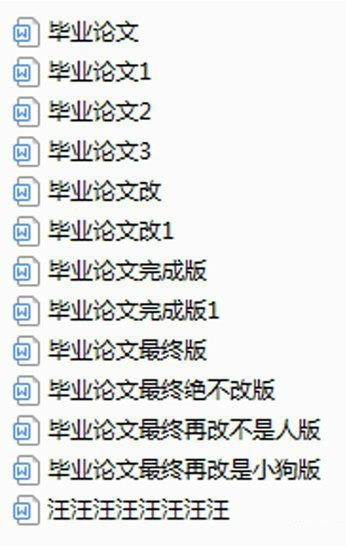
\includegraphics[width=0.95\columnwidth, right]{author-folder/Kai.Wu/thesis_versions.jpg}
    \end{figure}
\end{newminipage}

读到这里,你如果感兴趣可以做个实验,创建一个文件,里面写上一些内容。然后在其他文件夹新建一个同名文件,写上另一些内容。最后,把它拖过来,覆盖掉前面的文件,这时,试一试自己有没有任何办法找回前面文件的内容。

你可能要问,上面不是说了这么多备份方法吗?是的,这些备份方法主要的作用是防丢失,比如电脑丢失、硬盘损坏,但少有备份能做到防覆盖。比如,实时备份的网盘,你本地把文件错误覆盖了,云端也马上被覆盖了。本地备份硬盘,如果备份频率不高,则还有一线生机,但如果过一段时间再去找,也可能找不到了。

因此,为了你的论文(命根子)安全,完全值得再加一层保险:

\begin{enumerate}
    \item Windows开启系统级的文件历史保护:\url{https://www.asus.com.cn/support/FAQ/1013067/},别忘了一定要把你的论文文件夹添加进去才能生效
    \item mac的TimeMachine(时间机器)备份自带了文件历史功能。参照前面的 \ref{sec.pc_backup} 配置好TM,整个电脑的文件历史就都包括在备份里了。
    \item Linux用户,我相信你们有的是办法。最笨的办法,直接写一个shell脚本,把论文文件夹直接复制到其他目录、用日期命名,最后把这个脚本加到crontab里定期运行即可。
    \item 以上是开启本地文件历史的方法。一些网盘自带文件版本功能,但一般限制版本数量或者日期,或者必须要买会员才能开启文件版本。开启过后,相当于云端也存了一份版本历史,万一本地的你没设置好或者其他什么原因不能用,还能在错误覆盖的时候救你一命。学校的seadrive自带大概两个月的文件版本,免费,非常良心,再次建议大家使用。直接把文件夹拖进去备份,就会自动产生文件版本。参见章节 \ref{sec.net_drive_backup} 。
    \item 会一点Git、GitHub的同学,请直接把整个论文文件夹创建成Git项目,并上传到GitHub做成private repo,每天工作结束后交一个commit来备份版本,同时记录你修改了什么内容。对于论文,Git是最完美的备份方案,可以轻松回滚到老版本同时从不担心覆盖、甚至能轻松知道哪个地方的修改是在什么时候引入的,比以上所有方法都靠谱。Overleaf也有GitHub集成,可以方便的与导师协作。但Git学习成本略高,不过网上有无数详尽的教程,感兴趣、学有余力的同学可自行学习。
\end{enumerate}


\begin{flushright}
(2022年12月02日 by \Wu)

(major update: 2022年12月30日 by \Wu)
\end{flushright}

% \begin{figure}[H]
%     \centering
%     \includegraphics[width=0.5\columnwidth]{author-folder/Kai.Wu/}
% \end{figure}


% \usepackage[export]{adjustbox}

% \item 
% \begin{minipage}{0.3\textwidth}
%     文字
% \end{minipage}
% \begin{minipage}{0.63\textwidth}
%     \begin{figure}[H]
%         \includegraphics[width=0.95\columnwidth, right]{author-folder/Kai.Wu/}
%     \end{figure}
% \end{minipage}

% \input{author-folder/Kai.Wu/.tex}
 \clearpage

\section{Remote Control: How to Access Campus Computers from Off-Campus}

When you are off-campus, you might often miss your campus computer. Whether it's the desktop provided by the school or other computers bought with your advisor's funds, they can all be remotely controlled.

\subsection{Preparation for School-Provided Computers}
(If you are not trying to access a school-provided computer, please skip to the next section)

School-provided computers are quite special, and by default, we cannot install software on them. There are two ways to handle this:
\begin{enumerate}
    \item Email or call IT and directly ask for administrator privileges. Just say you are a PhD student and need to install software on the school-provided computer. After that, you can install the control software.
    \item After the above method, the computer is still managed by the school and there are still some restrictions, but it is generally sufficient for regular use. For those who want complete control over the school computer, you can format the disk and reinstall the system, or partition the disk (keeping the original system) and install a dual system. There are many tutorials on reinstalling Windows, partitioning, and setting up dual systems on Bilibili and Zhihu.
\end{enumerate}

\subsection{Recommended Desktop Control Software}
The following software can be used on any system: Windows, Linux, or Mac.
\begin{itemize}
    \item VNC: Install VNC Server on the controlled end (school computer) \url{https://www.realvnc.com/en/connect/download/vnc/}, and VNC Viewer on the controlling end (your computer) \url{https://www.realvnc.com/en/connect/download/viewer/}. Register an account and log in to use, no need to remember connection codes. Recommended because VNC is a well-tested remote desktop solution that generally works as long as the network is stable.
    \item ToDesk: \url{https://www.todesk.com/} Install the same software on both computers. Recommended because it is a new software and generally smoother than VNC.
    \item Others: AnyDesk, TeamViewer, Sunflower, all can be tried. However, TeamViewer is not highly recommended because it might detect the network environment of the school and force you to purchase a commercial version, which is not an issue with other software.
\end{itemize}

\subsection{Remote SSH}
(If you don't use Linux, you can skip to the next section on pitfalls)

If the controlled end is a Linux system and you mainly use command-line operations, connecting via SSH directly will be much faster than desktop control.

The computer on campus has an internal IP starting with 10. How to SSH from outside? This trick is called "NAT traversal."

First, I recommend this video:

\href{https://www.bilibili.com/video/BV1Qq4y1w7F5}{[Hardcore] Public Network Access? NAT Traversal! Zero Experience Start!}\url{https://www.bilibili.com/video/BV1Qq4y1w7F5}

The solutions available for campus machines in the video are:
\begin{itemize}
    \item At 04:52 in the video, using IPV6 connection. However, note that in my experience, the school's IPV6 is unstable and might stop working after a few days. Even if you can set up DDNS, I personally do not recommend it.
    \item A more reliable solution is introduced at 08:09 in the video: NAT traversal. Free and easy-to-use solutions include: Zerotier (slightly slow as it is overseas), Peanut Shell (an old domestic brand, but registration requires an ID card), NOFRP (new, reliability might be low), or directly search "free NAT traversal" on Bilibili for many new solutions. If you are not familiar with these, there are many tutorials on Bilibili and Zhihu.
    \item (Advanced high-traffic version, but with a higher learning curve) Free solutions have limitations on traffic and bandwidth, which are sufficient for SSH commands. But if you want to use SCP to transfer files or forward VNC via SSH, consider renting a cloud server with your advisor's funds and manually setting up an FRP service (a bit complicated, but very smooth once set up, faster than the previous remote desktop solutions). Alternatively, set up a junk machine as a jump server in your dorm with a public IP and DDNS for unlimited traffic access. These solutions have a higher learning curve, but you can refer to online tutorials and experiment slowly.
\end{itemize}

\subsection{Pitfalls}
Here are some experiences I gained after encountering many pitfalls:
\begin{enumerate}
    \item Redundancy to improve reliability: Do not rely on a single remote control solution. If one fails, you can use another. Please install at least two, and if you are away for a long time, install more. I personally use: a second-hand thin client at home with FRP and DDNS + Peanut Shell as a backup plan + VNC as another backup plan + ToDesk, a four-layer backup solution for stable access to my campus Linux computer.
    \item After installation, restart once to see if the control software can start automatically.
    \item If the controlled end is a Windows computer, be sure to disable system updates. Although restarting is fine, a major Windows update might get stuck on a screen asking you to agree to a new user agreement, and unless you are there to click it, no software will start, and you will lose control. Please search "disable Windows updates" on Baidu. I personally recommend using a combination of group policy and host file modification.
    \item For those running programs, be sure not to exceed memory limits or crash the system memory. If the memory is fully used, the system will crash immediately, killing all control software, and it will not restart automatically. You must be there to force a restart. Please find ways to monitor and control memory usage in your programs.
    \item If possible, purchase remote KVM hardware like "Sunflower Control" to force a remote restart even if the system crashes.
    \item No matter how good the solution is, it cannot prevent network maintenance or power outages on campus. These can be defended against. For network outages, make sure to check the macauth option when logging in to the network, so it will work again after maintenance. For power outages, the motherboard needs to support the "boot on power" or "boot with power" function. Check the motherboard manual or search for "power" to see if it is available. Alternatively, purchase Sunflower Control. However, power and network outages are rare, and unless you are away for months, you generally do not need to worry about them.
    \item Maintain a good relationship with at least one on-campus classmate. Newcomers will encounter various unexpected situations and lose control, requiring office classmates to help check the machine. Behind 100 remote control solutions, you also need good classmates for physical control. In case the network cable is accidentally kicked out, you still need a classmate to help you fix it.
\end{enumerate}

\begin{flushright}
(09 November 2022 by \Wu) \\
Translated by GPT
\end{flushright}
 \clearpage

\section{我的老腰受不了了——如何保持颈椎、腰椎健康}

\subsection{缓解腰的问题:升降桌}

\begin{newminipage}[0.39]
    \begin{figure}[H]
        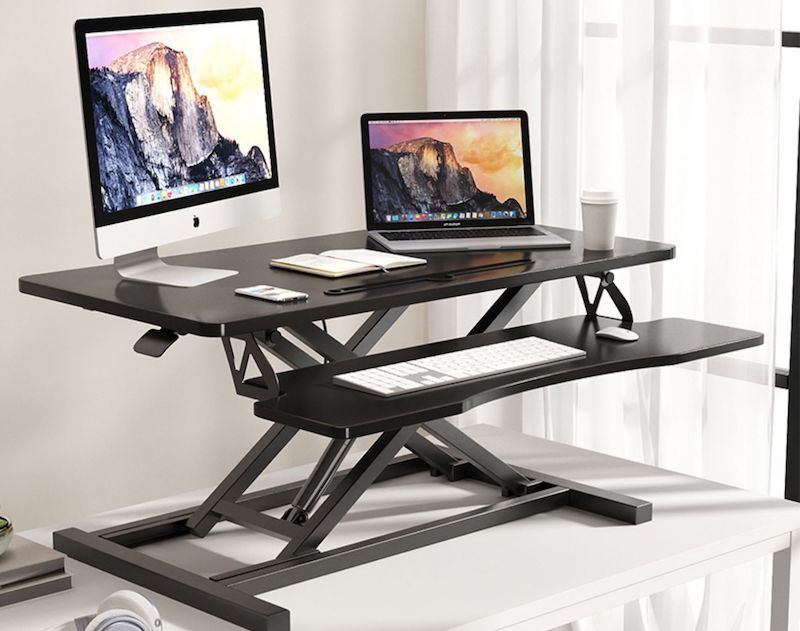
\includegraphics[width=0.95\columnwidth, right]{author-folder/Yue.Zhou/gongzuotai.jpg}
    \end{figure}
\end{newminipage}
\begin{newminipage}[0.6]
    在没有读博之前,我就患上了严重的腰肌劳损。这个玩意怎么说呢,说是大病吧,他不是,但无时无刻不在折磨着你。最严重的时候,疼的我晚上都睡不着。去医院看过也开过药,但医生说这个病需要自己保养,无法根治。后来我试着跑了半年步,哎!腰肌劳损神奇的好了,现在一点都不疼了(如遇久坐,仍旧是不行的,会疼)。读博之后也没有心情运动了,于是买了一个升降工作台(推荐人手一个!太好用了!)。可以站着办公,站累了就坐下办公。极大程度上杜绝了久坐对腰椎的伤害。
\end{newminipage}

\begin{flushright}
(2022年12月30日 by Yue Zhou)
\end{flushright}

\subsection{来自重度腰椎间盘突出、颈椎病患者的深度建议}

\subsubsection{升降桌:可极大缓解腰椎问题,但不能完全解决}

我十年腰椎间盘突出加五年颈椎病,19年的时候腰就疼到没法坐一整天,就在实验室放了台升降桌,站着用了三年电脑。今年还在卧室里放了同款升降桌。但长期站着和坐着一样对腰不好,最后会变成站着和坐着一样会腰疼。升降桌不是长久之计,站着只是换了角度继续损耗腰椎。

不能完全依赖升降桌:这几年太依赖升降桌,导致现在长时间站着和坐着一样腰疼,去拍核磁医生都问我是不是腰骨折了。如果真的想缓解腰疼,就要避免久坐久站。中学教师容易得腰疼一方面就是因为站着讲课时间长了。

总之升降桌可以用,但不能长期用它代替坐着用电脑。可以交替用,平时再多锻炼就行。

注意事项:升降桌记得没事调一调高度。我放实验室里的升降桌几年没调好像液压杆生锈了,都调不动了,直接变成了一般桌子。

\subsubsection{外接屏:避免和缓解颈椎病}

颈椎病难受的一点就是,低头时间长就脖子疼,出门在地铁高铁上我都不得不把手机竖起来抬高和眼平行,不然用不了太长时间。

我再贡献一个避免和缓解颈椎病的方法,就是不要长时间用笔记本电脑,长时间低头看屏幕会演变成颈椎病。低头看手机也是。

如果常用笔记本电脑就要在卧室和办公室都放一个台式机屏幕当外接屏。

我颈椎病就是高强度用了一年笔记本电脑得上的,后来只用外接屏就不再继续加重了。

如果经常高强度用笔记本电脑,不用外接屏的话和整天低头用手机一样都是颈椎杀手。我在实验室看见有人长时间用笔记本都会劝他们用外接屏。

笔记本支架也可以,比显示器便宜。但如果视力不好,还是尽量外接屏,因为笔记本屏幕太小了,费眼。我以前也买了很多笔记本支架,现在都用来放显示器了,笔记本刚好能放在下面很方便。

\begin{figure}[H]
    \caption{我自己在卧室里就是升降桌,配笔记本支架。这个组合很适合我这种主要用笔记本的}
    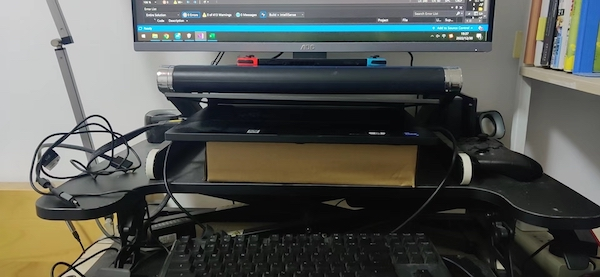
\includegraphics[width=0.95\columnwidth, center]{author-folder/Jialin.Wang/shengjiangzhuo.jpeg}
\end{figure}


% \subsubsection{进一步缓解:趴着用电脑}

% 我今年起站也不能站太长时间,已经开始探索平躺和俯卧用电脑了。平躺我试过几天就放弃了,容易睡着。我觉得平躺就适合看看电影玩游戏。

% 俯卧我最近试了一个月,感觉还行,起码支起上半身不会犯困。

% 我是放了一个便携屏幕在床边,然后配一个趴枕,这样能趴一整天。趴枕好处是吃完饭趴着不会压迫腹部导致不适。

% \begin{figure}[H]
%     % \centering
%     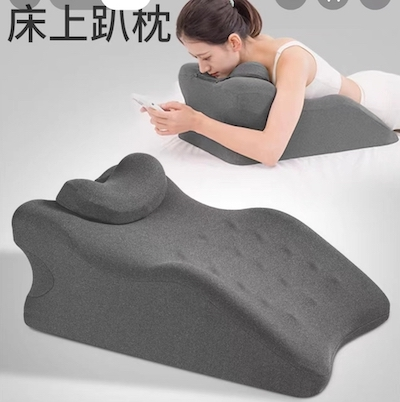
\includegraphics[width=0.3\columnwidth, center]{author-folder/Jialin.Wang/pazhen.jpeg}
% \end{figure}

% 然后配一个可以调角度的笔记本支架放屏幕键盘和鼠标——其实直接放笔记本也行,但发热量大,搬来搬去不方便。用便携屏能快速在升降桌和俯卧之间切换——我也想过买一般的显示器支架,但没有卖那种适合在床上用的,而且一般显示器在床上用太大了。便携屏就是笔记本二手屏幕改装的,大小和笔记本电脑一样在床上用正好。

% 如果长时间趴着用电脑,我发现最好是用双臂稍微用力撑起上半身。但上半身主要还是靠着躯干受力,双臂是辅助作用,避免下巴受力太大。

% 我现在已经练成了能俯卧一天的神功,笔记本支架只要调好角度,让手和手臂平行,这样手腕就不会因为长时间弯曲而酸痛。

% 不过最近因为趴习惯了加上天冷就完全不锻炼,如果不趴着,还是腰疼。还是得坚持锻炼才行。

% 这一套方案我觉得真的完美适合我这种腰疼到无法长时间坐着和站着的人,但这些都不能治好腰疼。锻炼才是最重要的。时间长不锻炼,不常用的肌肉会萎缩,更不好。(我好想以后住在热带沿海地区,每天傍晚去海边游泳,傍晚的时候海水是温的)


\subsubsection{最好的解决方案:改变生活习惯、加强锻炼}

建议有腰椎间盘突出和颈椎病的人还是多锻炼。但不要盲目去健身房锻炼,最好的锻炼方法还是游泳,因为其他锻炼方式大多会需要腰部用力,加重腰疼。

我目前只是偶尔腰疼到不能弯腰。我还认识腰疼到走路一瘸一拐的,他也是慢慢锻炼才逐渐好转。

如果自制力不强,加学校游泳社团也行,起码有人经常一起去锻炼能有动力。

办卡的话,我记得每年九月份独墅湖游泳馆能办半价年卡,但学校社团很便宜,更划算。以前我办游泳卡前每周都跟着学校游泳社团去游一两次,办了年卡后,一年去了不到五次,后来就去得更少了。
如果自制力可以,每天锻炼是最好的方法。
如果坚持不下去,还无法改变生活习惯,就会越来越严重。

最后,如果腰疼比较严重,有空可以去医院骨科看看,做一下核磁,看一下腰椎到底发展到哪个地步,来决定怎么具体该恢复。现在腰疼在年轻人里很普及。

\begin{flushright}
(2022年12月30日 by Jialin Wang)
\end{flushright} \clearpage

\section{Liverpool Visit}
\label{section.UoL_visit}

\subsection{Potential Opportunities}
\subsubsection{Collaboration with Liverpool Supervisors}
Although most students will have a supervisor from Liverpool on their team, each project may be different, and you may not have frequent interactions with them before going to Liverpool. This infrequency could be due to various reasons, not necessarily because your work is in a different field. So if you think it would be interesting to collaborate with them in Liverpool, please prepare in advance.

If you haven't had much interaction with them before, make sure to establish some familiarity through some means, which will make future collaboration smoother. This can be through video meetings or emails sharing your research progress and plans, co-authoring papers, or brainstorming potential collaborative research content in advance.

We know that teamwork can happen for different reasons (see \ref{subsection.teamwork}), but in any case, be sure to confirm at least the general direction of your activities during your visit with your Liverpool supervisor in advance, including but not limited to: things that require their involvement, schedule, things you need to prepare, and things you plan to do.

\subsection{Accommodation and Living}
\href{https://hallslife.liverpool.ac.uk}{Halls Life} is the community hub for student accommodation at the University of Liverpool, providing various suggestions on accommodation and living. It is strongly recommended to browse it before departing for the UK, as it can help decide whether to bring certain luggage.

\subsubsection{Visiting Other University Libraries}
When you are traveling and visiting various universities in the UK, if you happen to pass by a university library when you are tired, you can actually go in and sit down, as long as you have applied for \href{https://access.sconul.ac.uk/sconul-access}{SCONUL Access} in advance.

Although different libraries have different policies, in most cases, you can at least enter the library after successfully applying, and some libraries may also provide computer access or book borrowing privileges.

\begin{quote}
    Q. Do I need to complete an online application for each institution I would like to visit?
    
    A. No, although you do need to indicate a library you are interested in visiting as part of your application, your approval email allows you to visit any of those libraries on the list. You do not need to reapply. \hfill 21 Oct, 2024 from \href{https://access.sconul.ac.uk/page/access-faq#Multiple%20applications}{Access FAQ | SCONUL}
\end{quote}

After submitting the application, it will be processed by the University of Liverpool Library, and once approved, you can go to the front desk of each university library with the email to get a visitor card.

\subsection{Food and Entertainment}
\href{https://hallslife.liverpool.ac.uk}{Halls Life} is the community hub for student accommodation at the University of Liverpool, providing various suggestions on food and entertainment.

\begin{flushright}
    October 21, 2022 by \Shiyao

    Translated by GPT
\end{flushright}
 \clearpage

\section{XJTLU Virtual Machine}
\url{https://vdi.xjtlu.edu.cn/portal/webclient/index.html}
If you are outside the university and want to quickly access on-campus resources and software temporarily, you can use the university's online virtual machine. The virtual machine is equivalent to a computer located on campus.

\section{Library Literature Databases}
After connecting to the campus network, most of the journals subscribed by the university can be directly downloaded from the journal pages. However, (1) some journal websites cannot recognize your IP, such as the famous Annual Review series; (2) if you want to download papers off-campus, you can use the library's literature databases.

\begin{figure}[H]
    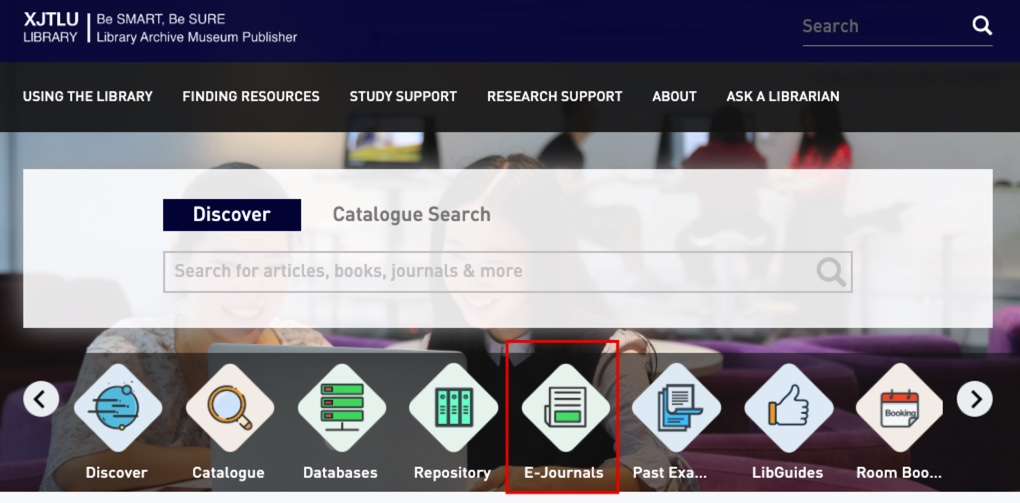
\includegraphics[width=0.7\columnwidth, center]{author-folder/Kai.Wu/library-ejournal.jpg}
\end{figure}

What I use most is clicking e-journal on the homepage \url{https://lib.xjtlu.edu.cn}, searching for the journal by name, and then accessing it through a dedicated link. The library also provides many full-text databases, including CNKI and other Chinese journal databases. For detailed usage, see the library's past training sessions \url{https://core.xjtlu.edu.cn/course/view.php?id=905}, or directly find the PPT in this project's GitHub (\href{https://github.com/xp-pgrs-unofficial-guide/xp_pgrs_unofficial_guide/tree/main/fileshare}{link}).

\section{Borrowing Books from Suzhou Library and Free Book Delivery}
If you want to read books from Dushu Lake Library or borrow books from Suzhou Library but don't want to go there because it's too far, what should you do? Just use the mini program to borrow books! Books from Suzhou Library can be \textbf{[free of charge]} delivered to Dushu Lake Library for pickup, and books from Dushu Lake Library can be directly delivered to the entrance of the university library.

Search for the mini program "Suzhou Library Borrow Books" on WeChat. Since the medical insurance card is the citizen card, you can use it to borrow books directly. If you have already obtained the medical insurance card, you can bind it directly to waive the card opening fee. Then follow the prompts in the mini program.

% \section{Student Medical Insurance}
\section{Pay Attention to Your Negative Emotions and Depression Tendencies}
\label{sec.mental_health}

\begin{figure}[H]
    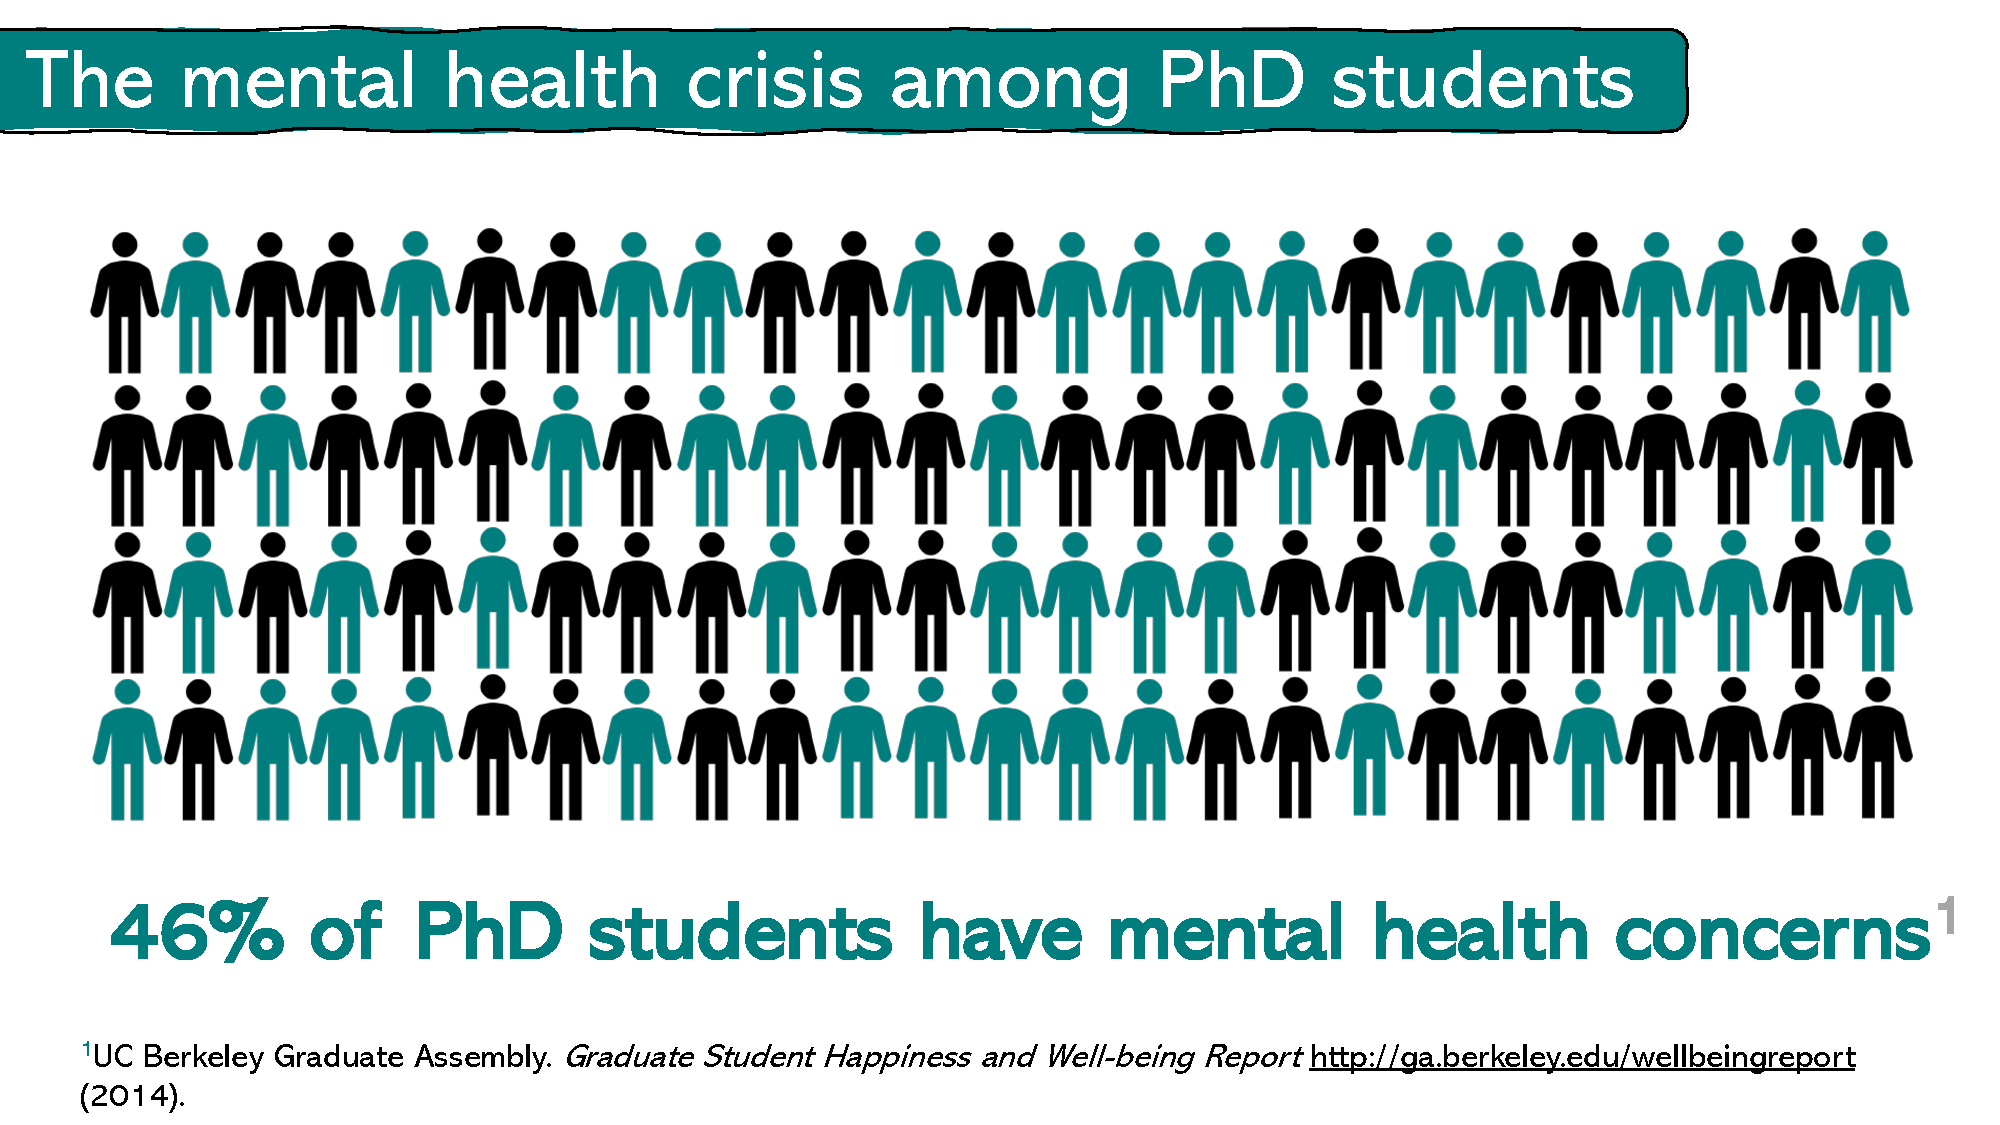
\includegraphics[width=0.6\columnwidth, center]{author-folder/Kai.Wu/mental_1.pdf}
    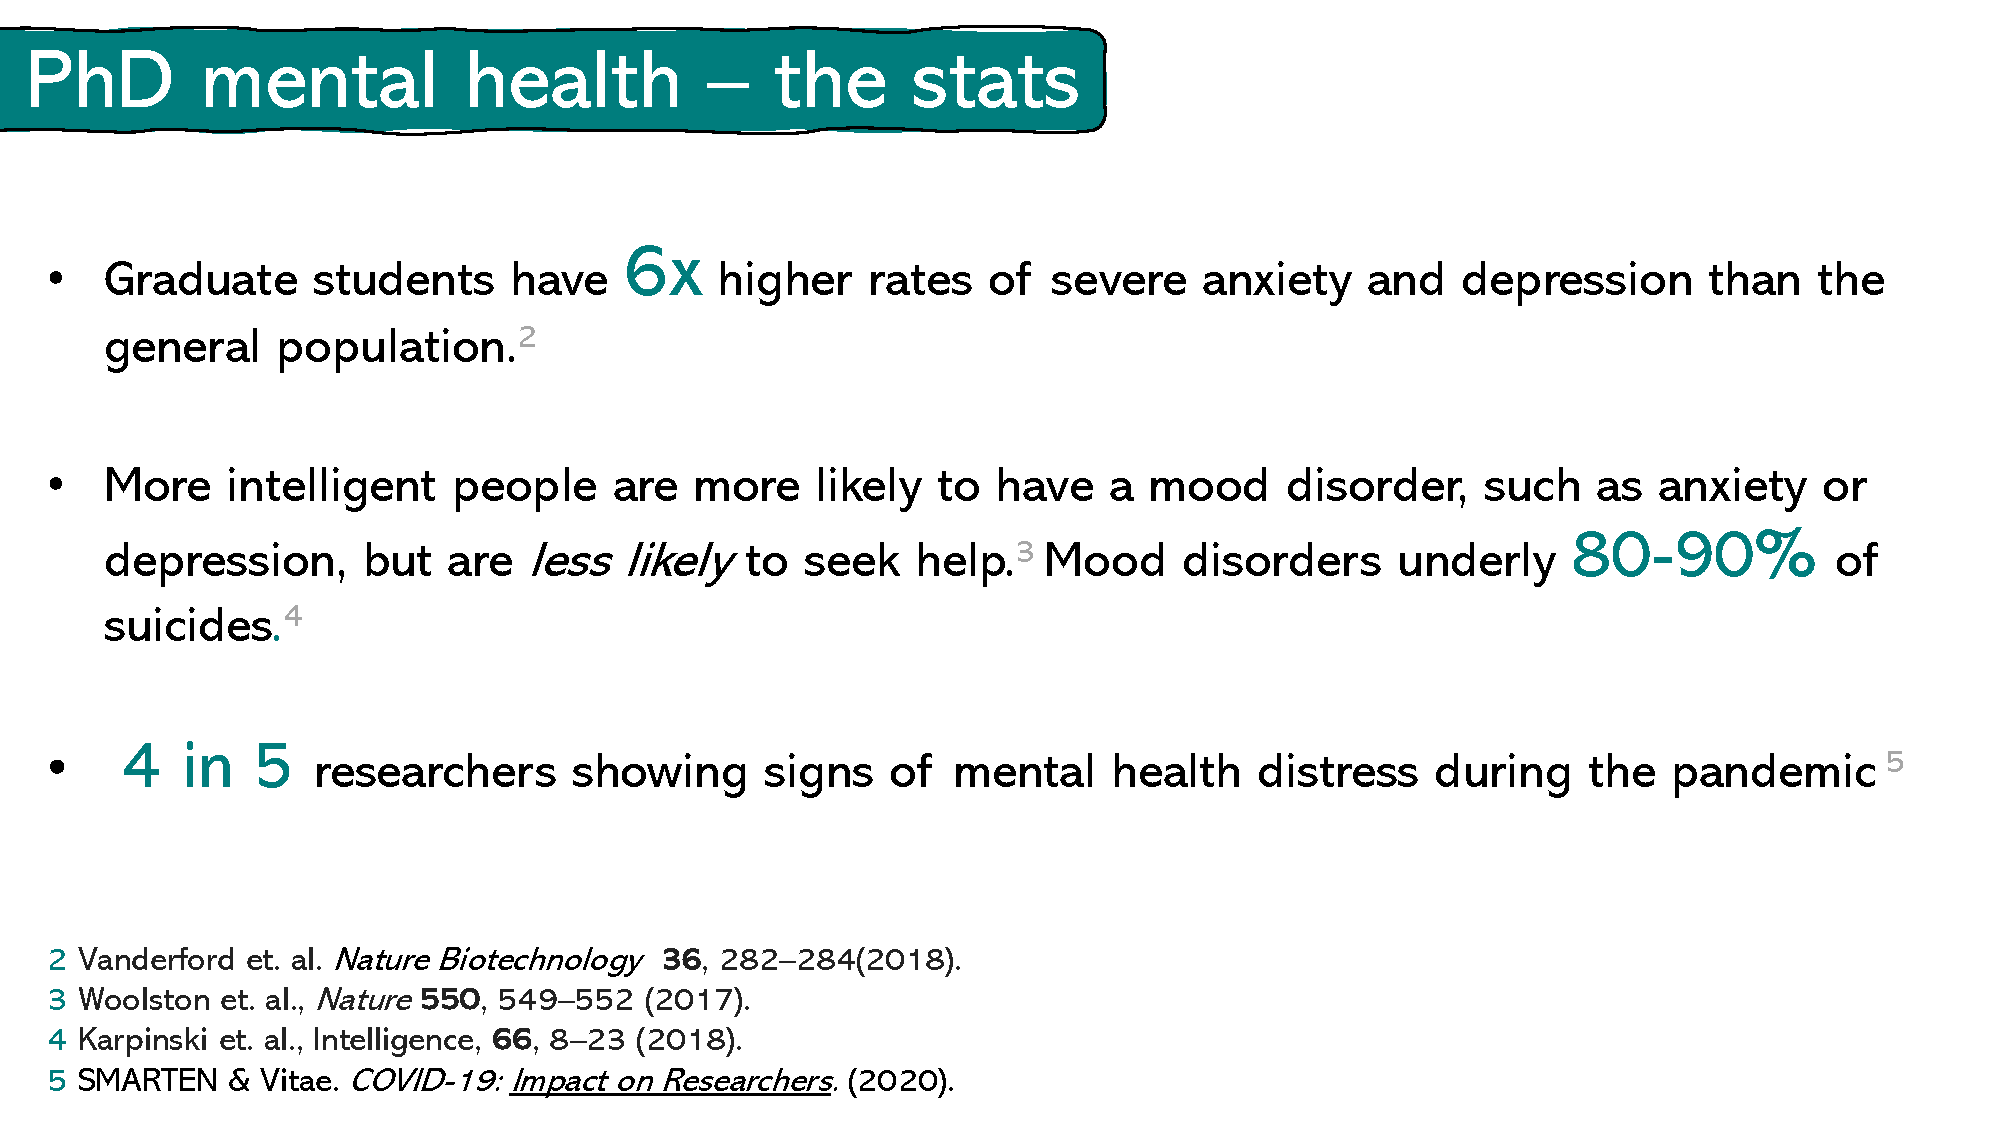
\includegraphics[width=0.6\columnwidth, center]{author-folder/Kai.Wu/mental_2.pdf}
    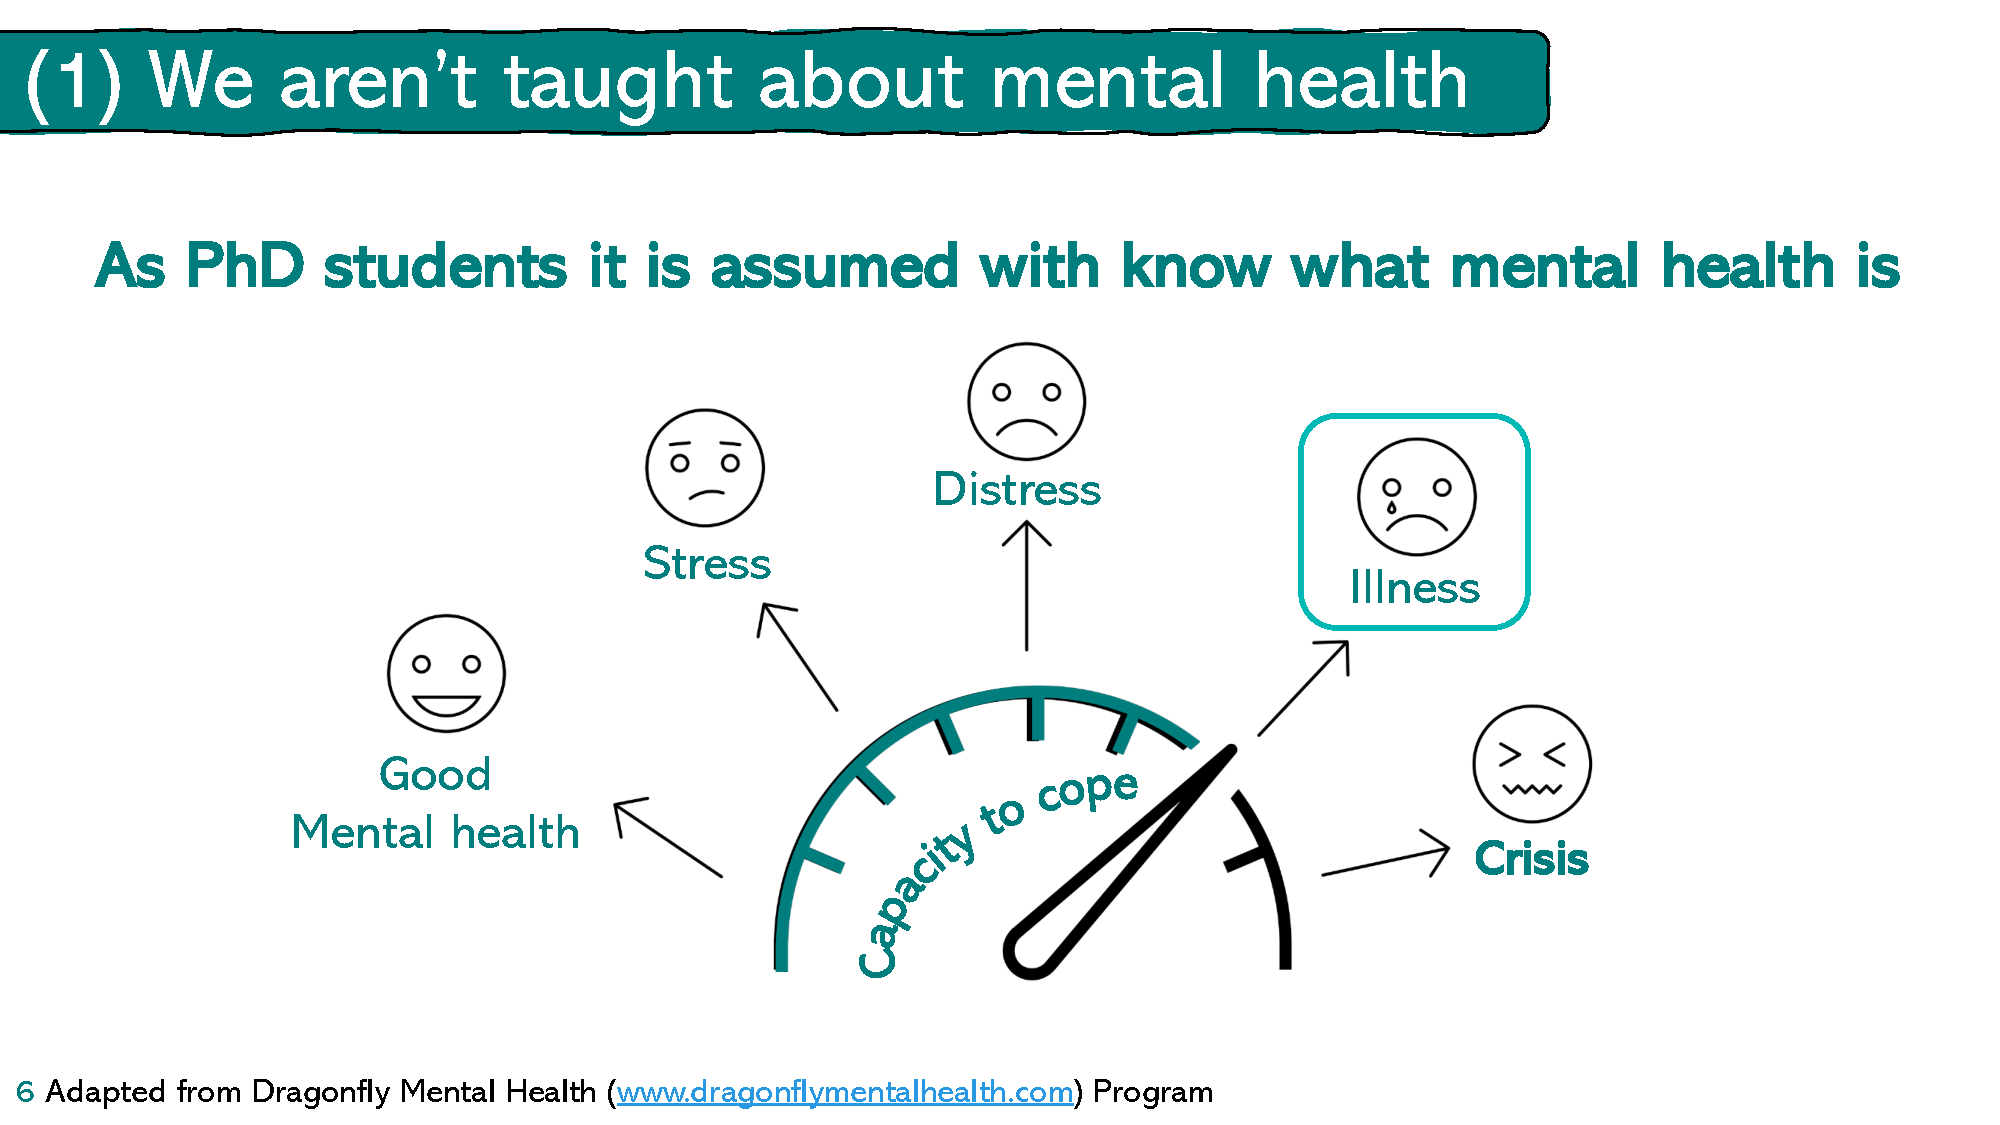
\includegraphics[width=0.6\columnwidth, center]{author-folder/Kai.Wu/mental_3.pdf}
\end{figure}

The \href{http://ga.berkeley.edu/wellbeingreport}{Graduate Student Happiness and Well-Being Report [link]} published by the Berkeley Graduate Assembly in 2014 shows that 46\% of Ph.D. students have mental health problems. Studies published in authoritative journals such as Nature suggest:
\begin{enumerate}
    \item Graduate students are six times more likely to suffer from severe anxiety and depression than the general population \href{https://www.nature.com/articles/nbt.4089}{[reference link]}
    \item Smarter people are more likely to suffer from mood disorders such as anxiety or depression but are less likely to seek help \href{https://www.nature.com/articles/nj7677-549a}{[reference link]}
    \item Mood disorders account for 80-90\% of suicides \href{https://www.sciencedirect.com/science/article/pii/S0160289616303324}{[reference link]}
    \item During the COVID-19 pandemic, four out of five researchers showed signs of mental health distress \href{https://www.tandfonline.com/doi/full/10.1080/21568235.2021.1992293}{[reference link]}
\end{enumerate}

\begin{figure}[H]
    \begin{tabular}{rcl}
        
\includegraphics[width=0.31\columnwidth]{author-folder/Kai.Wu/chat1of3.jpg} &
        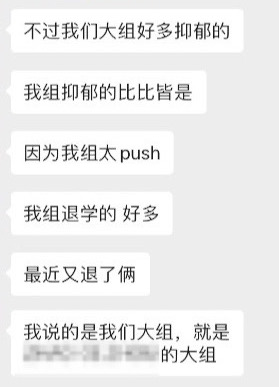
\includegraphics[width=0.31\columnwidth]{author-folder/Kai.Wu/chat2of3.jpg} &
        
\includegraphics[width=0.31\columnwidth]{author-folder/Kai.Wu/chat3of3.jpg}
    \end{tabular}
    \caption{Chat records with a graduated classmate. The incidence of depression among our university's Ph.D. students is higher than imagined}
\end{figure}

As a high-risk group, we have received extensive professional knowledge and skills training, yet almost no one has taught us "how to maintain mental health." If you often feel nervous, anxious, or disappointed now, and even have symptoms like insomnia, please immediately face your situation, put your health first, and feel free to seek help from the university's psychological counseling center.

Meanwhile, prevention is always more effective than post-treatment. I hope that everyone reading this, whether you feel good now or not, will click the links below, read Zoe Ayres' lecture in Liverpool (the source of the above PPTs), and her book "\textit{Managing Your Mental Health During Your PhD - A Survival Guide}," to get through your graduate studies healthily. ~~\href{https://github.com/xp-pgrs-unofficial-guide/xp_pgrs_unofficial_guide/tree/main/fileshare}{[GitHub link]}~~~~~\href{https://gitee.com/kaiwu-astro/xp_pgrs_unofficial_guide/tree/main/fileshare}{[Use this link if you can't access GitHub]}

\section{What Software Have You Installed on Your Computer? (Looking Forward to Your Additions)}

\KW: Let me start by sharing some software that I would definitely recommend to my fellow junior students:
\begin{figure}[H]
    
\includegraphics[width=\columnwidth]{author-folder/Kai.Wu/kai_mac_dock.jpg}
\end{figure}
\begin{itemize}
    \item Research and Productivity Tools
    \begin{enumerate}
        \item Notion (All platforms). An incredibly powerful new-generation note-taking app. I was originally a heavy OneNote user, but after being introduced to Notion by chance, I decided to abandon OneNote and completely switch to Notion after a short trial. Recommended because: supports Win/Mac/Linux/Web/iOS/Android; powerful database functions to perfectly build your own GTD system and greatly improve efficiency; fast global search; modern collaboration features, even usable for team and project management; powerful sharing features to easily share notes as public webpages; lots of tutorials on Bilibili.

        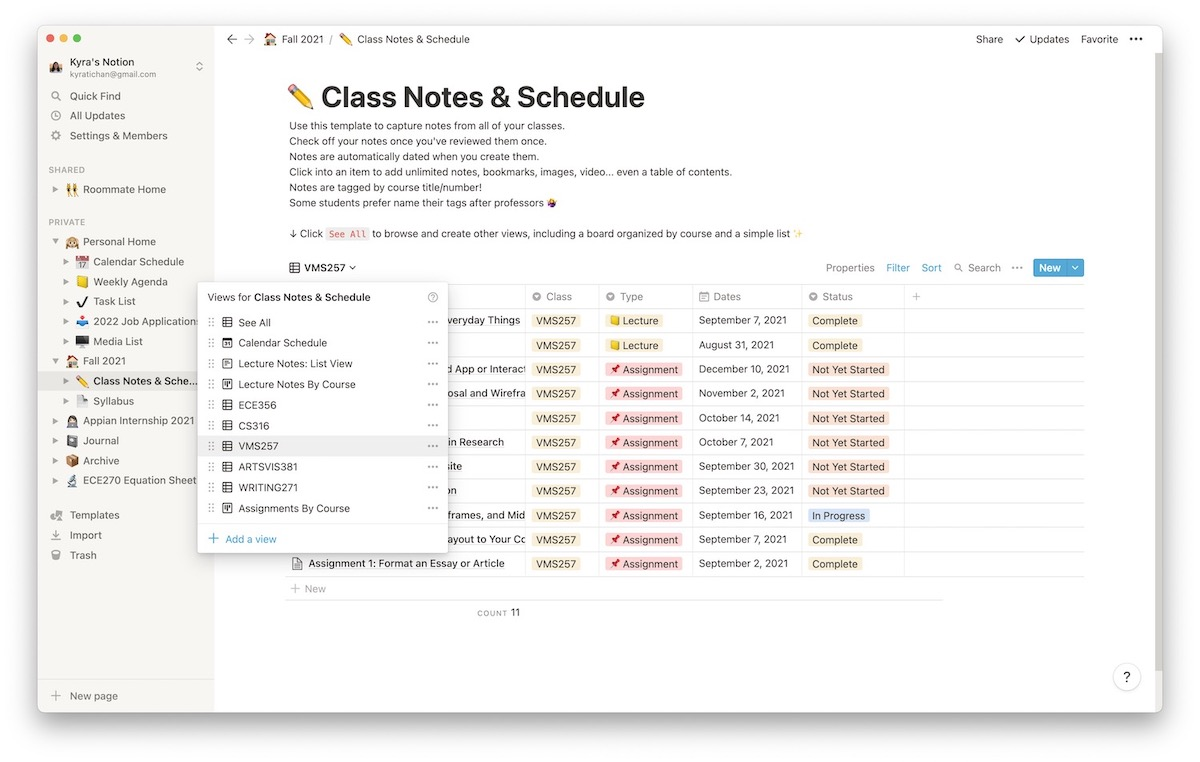
\includegraphics[width=0.8\columnwidth]{author-folder/Kai.Wu/notion.jpg}
        \item TickTick (All platforms). I've used Wunderlist (later acquired by Microsoft and became Microsoft To-Do), iOS's built-in Reminders, and several other list apps for a long time. Only TickTick feels the most intuitive and user-friendly. Used together with Notion, it can conveniently manage all aspects of study and life. Supports all platforms.

        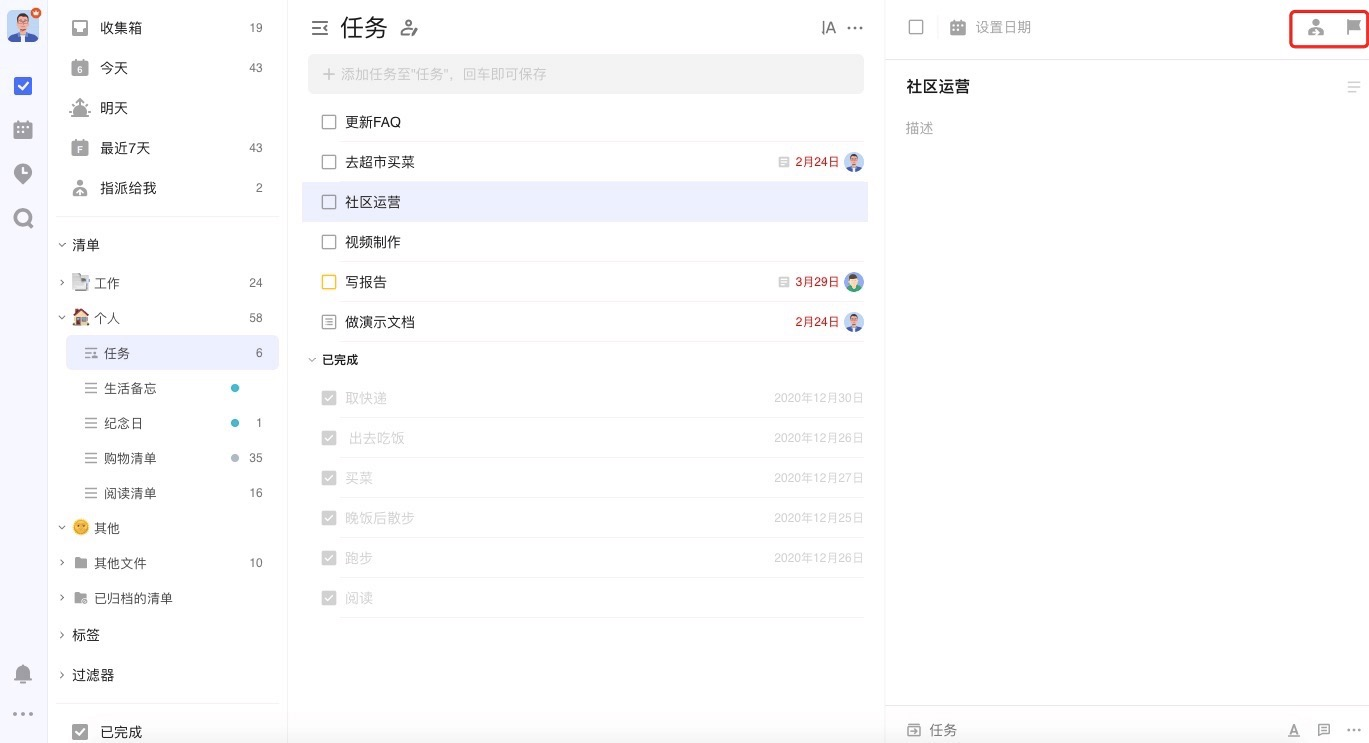
\includegraphics[width=0.8\columnwidth]{author-folder/Kai.Wu/dida.jpg}
        \item Trello (All platforms). Manage your to-do items and tasks with cards. My supervisor heavily relies on Trello to keep his numerous tasks well-organized. While I think Notion is a superset of Trello, if you don't like Notion for some reason, at least try Trello. Available for download on all platforms.

        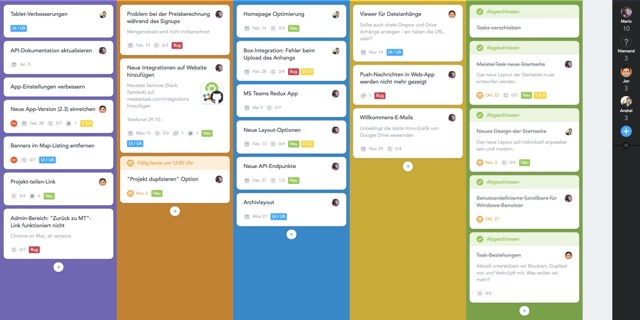
\includegraphics[width=0.8\columnwidth]{author-folder/Kai.Wu/trello.jpg}
        \item VSCode (Visual Studio Code) (All PC platforms). An open-source text editor that rose to prominence around 2019, with extremely strong community and plugin support. Currently, I use VSCode + LaTeX Workshop plugin for my journal papers, theses, and even this guide you're reading. All my numerical simulation programs and data analysis scripts are also done with VSCode. The drawbacks are a small learning curve and the need to configure settings; it also consumes memory like Chrome.

        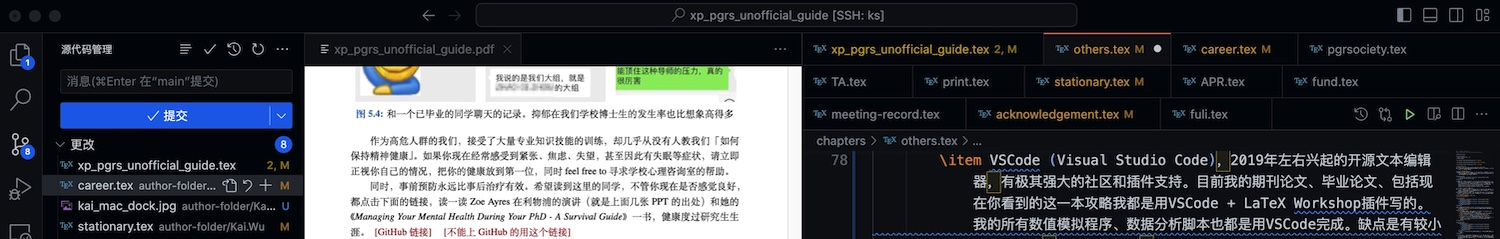
\includegraphics[width=0.8\columnwidth]{author-folder/Kai.Wu/vscode.jpg}
        \item Spark. An email app developed by Readdle, an award-winning Apple app developer, that manages all your email accounts in one place and syncs email settings to the cloud, solving the problem of re-adding multiple email accounts when you get a new device. It seems to be exclusive to Mac and iOS; not sure if it's available on other platforms.

        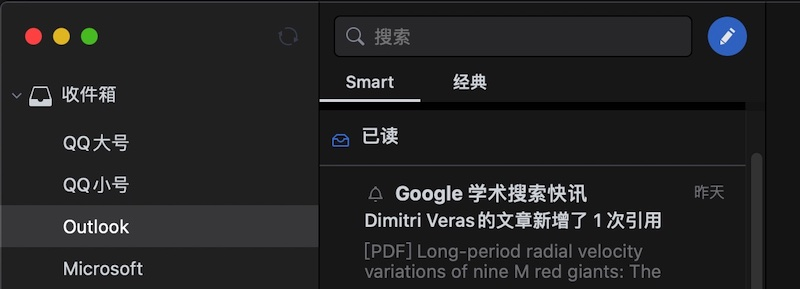
\includegraphics[width=0.8\columnwidth]{author-folder/Kai.Wu/spark.jpg}
        \item As for reference management software, I won't make recommendations—everyone has their own preferences. If you don't have one yet, ask your seniors or check out recommendations on Bilibili.
    \end{enumerate}
    \item Efficiency Tools
    \begin{enumerate}
        \item Bob (MacOS) or Pot (Win/Mac/Linux). Tools for word translation, screenshot translation, and OCR. Supports integration with ChatGPT, DeepL, Google Translate, Youdao Translate, and other translation services, and can even display results from multiple platforms simultaneously for comparison. Bob can be downloaded from the Mac App Store; Pot is available at pot-app.com.

        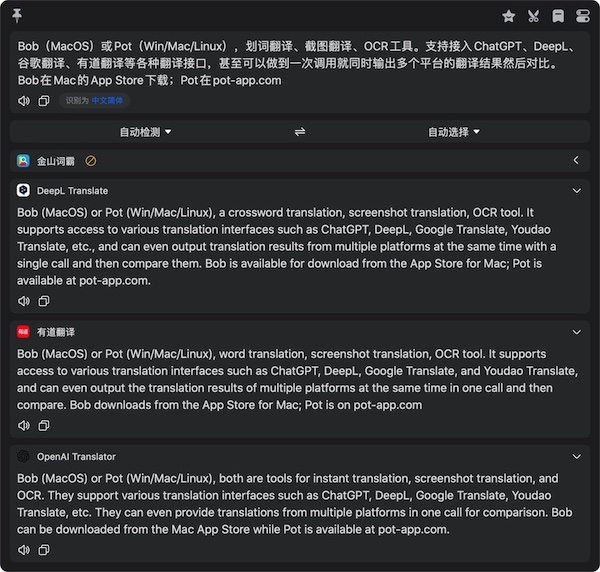
\includegraphics[width=0.8\columnwidth]{author-folder/Kai.Wu/Bob.jpg}
    \end{enumerate}
\end{itemize}

Have you discovered any great software? Please feel free to share them with your fellow junior students.

Your recommendations:

\begin{flushright}
    Translated by GPT
\end{flushright}